\chapter{Lợi suất và Phương sai Danh mục Đầu tư}
\label{ch:M3L1}

% Lesson: Portfolio Returns and Variance

\section*{Lesson Notes}

MODULE 3 | BÀI 1

{\small
\begin{longtable}{>{\raggedright\arraybackslash}p{0.213\linewidth}>{\raggedright\arraybackslash}p{0.727\linewidth}}
\toprule
\textbf{Thời gian đọc} & 2 giờ \\
\addlinespace[2pt]
\textbf{Kiến thức nền tảng} & Python, lợi suất, phương sai, đa dạng hóa \\
\addlinespace[2pt]
\textbf{Từ khóa} & Lợi suất, logarit, phần trăm, ký hiệu ma trận, phân phối, chuẩn hóa theo năm, trung bình hình học, trung bình số học, phương sai danh mục đầu tư, tương quan, trọng số \\
\addlinespace[2pt]
\bottomrule
\end{longtable}
}

\emph{Trong bài học này, chúng ta sẽ khám phá các loại lợi suất khác nhau, các phương pháp chuẩn hóa lợi suất theo năm, và các kỹ thuật tính phương sai danh mục đầu tư. Bài học nhằm mang lại một hiểu biết toàn diện về cách đo lường và diễn giải hiệu suất danh mục đầu tư, xét trên cả hai khía cạnh lợi suất và rủi ro.}

\emph{Chúng ta sẽ bắt đầu bằng việc xem xét các loại lợi suất khác nhau, bao gồm lợi suất phần trăm và lợi suất logarit, đồng thời thảo luận về đặc tính và trường hợp sử dụng phù hợp của từng loại. Sau đó, chúng ta sẽ chuyển sang các phương pháp chuẩn hóa lợi suất theo năm, điều rất quan trọng khi so sánh các khoản đầu tư qua các khoảng thời gian khác nhau. Bài học cũng sẽ đề cập đến cách tính phương sai danh mục đầu tư, khám phá cách phương sai của từng tài sản, trọng số và tương quan đóng góp vào rủi ro tổng thể của danh mục.}

\section{Lợi suất Danh mục Đầu tư}

Trong môn Thị trường Tài chính, bạn đã được giới thiệu về lợi suất tài sản và lợi suất danh mục đầu tư. Trong Dữ liệu Tài chính, chúng ta sẽ khám phá cả tập dữ liệu một chiều lẫn nhiều chiều. Do đó, biểu diễn ma trận trong đại số tuyến tính sẽ là cánh cửa chính để xử lý chủ đề này. Điều này hợp lý vì một danh mục đầu tư gồm $n$ tài sản với lợi suất $r_{i}, i \in \{1,n\}$ có thể được sắp xếp thành một ma trận $r$ trong đó mỗi cột đại diện cho một tài sản. Trong ngữ cảnh này, $r_{i}$ là các vector, và \textbf{khi không có hiện tượng đa cộng tuyến hoàn hảo}, ta có $\text{dim}(\text{span}(r_{i})) = n$.

Chúng ta đã biết rằng lợi suất danh mục đầu tư là:
$$
r_{p} = \sum_{1}^{n} w_{i} \cdot r_{i}
$$
trong đó
\begin{itemize}
  \item $r_{p}$: lợi suất danh mục đầu tư
  \item $r_{i}$: lợi suất của tài sản $i$
  \item $w_{i}$: trọng số của tài sản $i$
\end{itemize}

Chúng ta cần lưu ý thêm một ràng buộc:
$$
\sum_{1}^{n} w_{i} = 1
$$

và với mục đích của bài học này, chúng ta cũng giả định rằng không được phép bán khống (shorting):
$$
w_{i} > 0
$$

Về bản chất, lợi suất danh mục đầu tư $r_{p}$ là một tổ hợp tuyến tính của lợi suất từng tài sản. Theo cách xây dựng, ta có $r_{p} \in \text{span}(r_{i})$ với mọi tổ hợp trọng số. Điều đó có nghĩa là các tài sản mà nhà đầu tư lựa chọn chính là cơ sở (basis, theo nghĩa Đại số Tuyến tính) của danh mục đầu tư.

Bây giờ hãy viết lợi suất danh mục đầu tư theo định dạng mà chúng ta sẽ sử dụng trong suốt bài học và làm rõ ký hiệu:

$$
r_{p} = \mathbf{r} \cdot \mathbf{w}
$$

với
$$ \mathbf{r} = \begin{bmatrix} r_1 & r_2 & \dots & r_n \end{bmatrix} \text{ , } \mathbf{w} = \begin{bmatrix} w_1 \\ w_2 \\ \vdots \\ w_n \end{bmatrix}$$

và mỗi $r_{i}$ là một vector đại diện cho lợi suất của từng tài sản theo thời gian $t$:
$$
r_{i} = \begin{bmatrix} r^i_{t_{1}} \\ r^i_{t_{2}} \\ \vdots \\ r^i_{t_{m}} \end{bmatrix}
$$

Việc sử dụng $1$ làm tổng của tất cả các trọng số có một cách giải thích trực quan: chúng ta xây dựng danh mục đầu tư bằng cách sử dụng một tỷ lệ phần trăm của mỗi tài sản (các trọng số) cho đến khi dùng hết toàn bộ số vốn ($1$ nghĩa là $100\%$). Vậy điều gì sẽ xảy ra nếu ràng buộc đó bị phá vỡ?

\textbf{Bài tập 1:}

Sử dụng giáo trình tài chính yêu thích của bạn cùng các nguồn trực tuyến để tìm hiểu về ràng buộc $\sum_{1}^{n} w_{i} = 1$. Điều đó sẽ có ý nghĩa gì đối với một danh mục đầu tư nếu $\sum_{1}^{n} w_{i} = 2$? Trả lời câu hỏi tương tự nhưng lần này với $\sum_{1}^{n} w_{i} = 0$. Khởi tạo một chủ đề thảo luận trên diễn đàn để giải thích hiểu biết của bạn.

Hãy tải xuống một số dữ liệu thực tế:

\begin{lstlisting}[language=Python,escapeinside={(*@}{@*)}]
import numpy as np
import pandas as pd
import matplotlib.pyplot as plt
import seaborn as sns
sns.set()
\end{lstlisting}

\begin{lstlisting}[language=Python,escapeinside={(*@}{@*)}]
assets = ['MSFT', 'AAPL', 'AMZN', 'TSLA', 'GOOGL'] # (*@Các@*) (*@tài@*) (*@sản@*) (*@trong@*) (*@danh@*) (*@mục@*)
w = np.array([0.1, 0.2, 0.1, 0.4, 0.2]) # (*@Trọng@*) (*@số@*) (*@của@*) (*@mỗi@*) (*@tài@*) (*@sản@*)

asset_prices = pd.read_csv("portfolio_prices.csv", index_col = "Date", parse_dates = True)

r = asset_prices.pct_change().dropna() # (*@Tính@*) (*@lợi@*) (*@suất@*) (*@phần@*) (*@trăm@*) (*@hàng@*) (*@ngày@*)

r.head() # (*@Mỗi@*) (*@cột@*) (*@là@*) (*@một@*) $r_{i}$
\end{lstlisting}

\begin{lstlisting}[escapeinside={(*@}{@*)}]
                AAPL      AMZN     GOOGL      MSFT      TSLA
Date
2018-01-03 -0.000174  0.012775  0.017061  0.004654 -0.010233
2018-01-04  0.004645  0.004476  0.003884  0.008802 -0.008290
2018-01-05  0.011385  0.016163  0.013260  0.012398  0.006230
2018-01-08 -0.003714  0.014425  0.003531  0.001020  0.062638
2018-01-09 -0.000115  0.004676 -0.001274 -0.000680 -0.008085
\end{lstlisting}

\begin{lstlisting}[language=Python,escapeinside={(*@}{@*)}]
r_port = r @ w # (*@Tạo@*) (*@lợi@*) (*@suất@*) (*@danh@*) (*@mục@*) (*@đầu@*) (*@tư@*)
r_port.name = 'portfolio_returns'
r_port.head()
\end{lstlisting}

\begin{lstlisting}[escapeinside={(*@}{@*)}]
Date
2018-01-03    0.004059
2018-01-04    0.003611
2018-01-05    0.011902
2018-01-08    0.015802
2018-01-09   -0.001093
Name: portfolio_returns, dtype: float64
\end{lstlisting}

\section{Các Loại Lợi suất}

Trong ví dụ trên, chúng ta đã trình bày về bản chất một cách để tính lợi suất phần trăm hàng ngày của danh mục đầu tư. Nhưng đây không phải là loại lợi suất duy nhất được sử dụng trong thực tế:

\subsection{Lợi suất Phần trăm}

Lợi suất phần trăm, còn gọi là lợi suất đơn giản hoặc lợi suất số học, thường được sử dụng trong thực tế:
$$
r_{t} = \frac{p_{t} - p_{t-1}}{p_{t-1}}
$$
trong đó $p_{t}$ là giá của một tài sản tại thời điểm $t$.

Ưu điểm lớn nhất khi sử dụng loại lợi suất này là cách diễn giải trực quan: chúng thể hiện trực tiếp mức thay đổi phần trăm về giá trị. Nhược điểm là chúng không có tính cộng dồn theo thời gian đối với một tài sản, mặc dù chính vì lý do đó mà chúng lại thường được dùng với danh mục đầu tư.

Hệ quả của tính không cộng dồn này khá đơn giản để minh họa: giả sử bạn có một tài sản giá $A$. Tháng đầu tiên, giá tăng $20\%$, nhưng đến cuối tháng thứ hai, giá giảm $18\%$. Nếu lợi suất có tính cộng dồn, ta có thể cộng đơn giản $20\% - 18\% = 2\%$ và cho rằng tổng lợi suất trong 2 tháng là $2\%$. Nhưng như chúng ta sẽ thấy ở phần sau, điều đó không đúng.

Cuối cùng, lợi suất đơn giản không đối xứng. Không có giới hạn trên, nhưng lại có giới hạn dưới. Về mặt trực quan, lợi suất của một cổ phiếu không thể nhỏ hơn $-100\%$ vì giá sẽ trở thành số âm. Ngược lại, ở chiều tăng, lợi suất có thể lên rất cao, đặc biệt khi xét trên khung thời gian dài. Một cách khác để minh họa điều này: giá của một tài sản trong ba tháng liên tiếp là 100 -> 120 -> 100. Cuối tháng thứ hai, lợi suất là $20\%$, nhưng cuối tháng thứ ba, lợi suất là $-16.6\%$. Nếu lợi suất đơn giản đối xứng, thì cần cùng một giá trị tuyệt đối của lợi suất để đi từ 100 lên 120 rồi quay lại 100.

\textbf{Bài tập 2:}

Viết một hàm Python tùy chỉnh, nhận vào một mảng giá (ví dụ \texttt{asset\_prices['MSFT']}), và trả về mảng lợi suất số học. Bạn không được phép sử dụng bất kỳ hàm Python có sẵn nào. Đối chiếu kết quả với kết quả tạo ra bởi hàm \texttt{pct\_change} của pandas.

\subsection{Lợi suất Logarit}

Lợi suất log, còn gọi là lợi suất kép liên tục (continuously compounded returns), sử dụng logarit tự nhiên theo cách sau:

$$
r_{t_\text{log}} = ln \left ( \frac{p_t}{p_{t-1}} \right )
$$

Khác với lợi suất phần trăm, lợi suất log có tính cộng dồn theo thời gian đối với một tài sản:
$$
r_{(t_{i}-t_{j})_{\text{log}}} = \sum_{t = i}^{t = j} r_{t_\text{log}}
$$
chúng cũng thường được giả định (không phải lúc nào cũng đúng) là phân phối chuẩn, một giả định quan trọng cho nhiều mô hình kinh tế lượng và ngẫu nhiên.

Tính cộng dồn này chính là lý do cho tên gọi "lợi suất kép liên tục", vì giờ đây bạn có thể tính tổng lợi suất qua một khoảng thời gian dài chỉ đơn giản bằng cách cộng các lợi suất log trong từng giai đoạn con. Tuy nhiên điều này lại tạo ra một vấn đề: nếu chúng ta có lợi suất logarit riêng lẻ của nhiều tài sản, liệu có hợp lý khi dùng chúng để tính lợi suất của danh mục đầu tư hay không? Nếu việc cộng lợi suất log là một quá trình tính lãi kép, liệu ta có được phép cộng lợi suất log của các tài sản khác nhau?

Câu trả lời cho các câu hỏi trên là \textbf{không}, và ta cần đặc biệt lưu ý để sử dụng đúng loại lợi suất cho từng trường hợp.

Cuối cùng, lợi suất log có tính đối xứng. Về mặt toán học, ta có thể thấy:

$$
log \left ( \frac{p_{t}}{p_{t-1}} \right ) = - log \left ( \frac{p_{t-1}}{p_{t}} \right )
$$

Sử dụng các con số trong ví dụ trên, ta thấy lợi suất log từ 100 lên 120 có giá trị bằng (nhưng ngược dấu) với lợi suất log từ 120 về 100.

\textbf{Bài tập 3:}

Viết một hàm Python tùy chỉnh, nhận vào một mảng giá (ví dụ \texttt{asset\_prices['MSFT']}), và trả về mảng lợi suất logarit.

Như đã minh họa ở trên, chúng ta chỉ có thể phân biệt hai loại lợi suất này dựa trên trường hợp sử dụng. Nhưng bây giờ chúng ta cần cụ thể hơn về thời điểm và cách thức. Để làm điều đó, chúng ta cần thực hiện một quan sát:

\begin{lstlisting}[language=Python,escapeinside={(*@}{@*)}]
print("The 25th quantile is: ", r['MSFT'].quantile(0.25),"\nThe 75th quantile is: ", r['MSFT'].quantile(0.75))
\end{lstlisting}

\begin{lstlisting}[escapeinside={(*@}{@*)}]
The 25th quantile is:  -0.008331217592874807
The 75th quantile is:  0.01093808706491084
\end{lstlisting}

Kết quả trên minh họa rằng, trong nhiều trường hợp, lợi suất hàng ngày có bậc độ lớn khoảng $1\%$. Ngoài ra, đối với lợi suất logarit và lợi suất phần trăm, ta có:
$$
r_{\text{log}} = ln \left ( \frac{p_{t}}{p_{t-1}} \right ) =
ln \left ( \frac{p_{t} - p_{t-1} + p_{t-1}}{p_{t-1}} \right ) =
ln (1 + r_{\text{pct}})
$$

Sử dụng khai triển Taylor cho công thức trên, ta được:
$$
r_{\text{log}} = ln (1 + r_{\text{pct}}) = r_{\text{pct}} - \frac{r_{\text{pct}}^2}{2} + \frac{r_{\text{pct}}^3}{3} - \frac{r_{\text{pct}}^4}{4} + \dots
$$

Vì chúng ta đã quan sát rằng lợi suất hàng ngày nhỏ $< 0.01$, ta có thể giả định rằng các số hạng bậc cao hơn ($r_{\text{pct}}^3$ trở lên) sẽ rất nhỏ:

$$
r_{\text{log}} = r_{\text{pct}} - \frac{r_{\text{pct}}^2}{2} + O(R^3)
$$

Lấy kỳ vọng của cả hai vế trong công thức trên và thực hiện các phép biến đổi đại số, ta có:

$$
\mathbb{E}(r_{\text{log}}) \approx \mathbb{E}(r_{\text{pct}}) - \frac{\sigma^2}{2}
$$
trong đó $\sigma$ là phương sai của lợi suất phần trăm.

Kết quả trên minh họa hai sự thật quan trọng:
\begin{enumerate}
  \item Khi độ biến động thấp, ta kỳ vọng lợi suất log và lợi suất phần trăm sẽ rất gần nhau (Ruppert và Matteson).
  \item Khi tần suất lấy mẫu giảm xuống, lợi suất log và lợi suất phần trăm có xu hướng lớn hơn về giá trị tuyệt đối, và do đó độ biến động cũng có xu hướng tăng lên. Điều này dẫn tới sự phân kỳ giữa hai loại lợi suất.
\end{enumerate}

\begin{lstlisting}[language=Python,escapeinside={(*@}{@*)}]
# Figure 1

pct_returns_msft = asset_prices['MSFT'].pct_change().dropna() # (*@Tính@*) (*@lợi@*) (*@suất@*) (*@phần@*) (*@trăm@*)
log_returns_msft = np.log(asset_prices['MSFT'] / asset_prices['MSFT'].shift(1)).dropna() # (*@Tính@*) (*@lợi@*) (*@suất@*) log

pct_change_msft_roll_mean = pct_returns_msft.rolling(15).mean() # (*@Trung@*) (*@bình@*) (*@trượt@*) (*@của@*) (*@lợi@*) (*@suất@*) (*@phần@*) (*@trăm@*)
log_returns_msft_roll_mean = log_returns_msft.rolling(15).mean() # (*@Trung@*) (*@bình@*) (*@trượt@*) (*@của@*) (*@lợi@*) (*@suất@*) log

fig, ax = plt.subplots(figsize=(12,4))
ax.set_title('Difference between pct and log returns vs Price of MSFT')
ax.plot(asset_prices['MSFT'], label = 'MSFT Price', alpha = 0.7)
ax.set_ylabel('Price')
ax.set_xlabel('Date')
ax.legend()

ax2 = ax.twinx()
ax2.plot((pct_change_msft_roll_mean - log_returns_msft_roll_mean), color = 'red', alpha = 0.5, label = 'Difference between pct and log returns')
ax2.set_ylabel('Difference')
ax2.legend(loc = (0.01,0.89))
plt.show()
\end{lstlisting}

\begin{figure}[H]
\centering
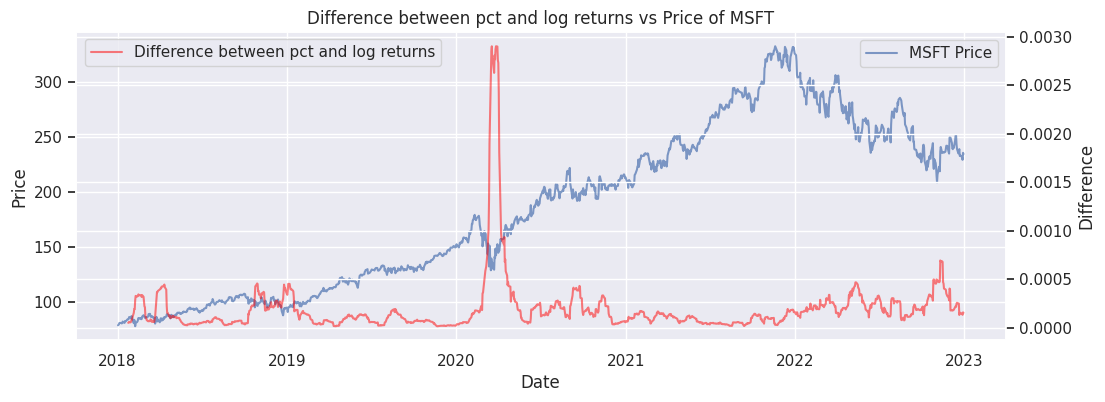
\includegraphics[width=\linewidth,height=0.6\textheight,keepaspectratio]{gfx/m3l1_notes_fig1_pct_vs_log_returns_msft.png}
\par\smallskip{\small \textbf{Hình 1.1:} Chênh lệch giữa lợi suất phần trăm và lợi suất log so với giá MSFT}
\end{figure}

Hình 1.1 minh họa sự chênh lệch giữa lợi suất phần trăm và lợi suất log. Trong các giai đoạn biến động thấp, hai loại lợi suất rất gần nhau, trong khi trong giai đoạn thị trường sụp đổ tháng 3/2020, chênh lệch này trở nên rõ rệt.

\textbf{Bài tập 4:}

MSFT là một cổ phiếu có độ biến động thấp. Hãy tái tạo Hình 1.1 nhưng lần này sử dụng TSLA để minh họa rõ ràng giai đoạn nào hai loại lợi suất phân kỳ.

\textbf{Bài tập 5:}

Hãy lập luận vì sao việc tính trung bình số học có trọng số của lợi suất log của các tài sản khác nhau tại một thời điểm cụ thể sẽ không cho ra lợi suất danh mục đầu tư tại thời điểm đó.

\textbf{Bài tập 6:}

Sử dụng DataFrame \texttt{asset\_prices} đã cho, tính giá trị danh mục đầu tư hàng ngày bằng cách tính tổng có trọng số của giá các tài sản, sử dụng trọng số tài sản đã định trước (như khi tính lợi suất danh mục đầu tư). Tiếp theo, tính lợi suất logarit của chuỗi giá trị danh mục đầu tư này. Thảo luận về các trường hợp sử dụng tiềm năng và ưu điểm của việc dùng lợi suất log trong ngữ cảnh này.

\textbf{Bài tập 7:}

Sử dụng DataFrame \texttt{asset\_prices} đã cho, tính lợi suất lũy kế của mỗi tài sản trong toàn bộ giai đoạn bằng ba phương pháp khác nhau:

\begin{enumerate}
  \item Sử dụng mảng lợi suất phần trăm hàng ngày của mỗi tài sản (gợi ý: bạn sẽ cần dùng hàm \texttt{prod}).
  \item Sử dụng lợi suất log hàng ngày.
  \item Sử dụng mảng giá tài sản.
\end{enumerate}

\section{So sánh Lợi suất Hình học và Số học}

Chúng ta sẽ tiếp tục thảo luận từ Module 2 về cách chuẩn hóa lợi suất theo năm, nhưng trước khi đi sâu vào chủ đề này, chúng ta sẽ xem xét một ví dụ đơn giản minh họa loại trung bình nên được sử dụng cho từng loại lợi suất, \textbf{nếu hiệu ứng lãi kép của lợi suất là cần thiết}.

\subsection{Ví dụ về Trung bình Hình học}

Giả sử tại thời điểm $t_{0}$, bạn có 100 đơn vị. Giữa $t_{0}$ và $t_{1}$, lợi suất của bạn là 20\%, và giữa $t_{1}$ và $t_{2}$, lợi suất là -18\%. Ta giả định các $t_{i}$ cách đều nhau.

\textbf{Tính Trung bình Số học}

Trung bình số học của lợi suất là:

$$
r_{\text{mean}} = \frac{0.2 - 0.18}{2} = 0.01
$$

Điều này cho thấy, trung bình mỗi giai đoạn lợi suất là +1\%. Theo logic này, trong giai đoạn đầu tiên, ta sẽ kiếm được:

$$
100 \cdot 0.01 = 1 \text{ đơn vị}
$$

Vậy, cuối giai đoạn đầu tiên, ta sẽ có 101 đơn vị. Trong giai đoạn thứ hai, giả sử vẫn lợi suất +1\%:

$$
101 \cdot 0.01 = 1.01 \text{ đơn vị}
$$

Điều này ngụ ý rằng cuối giai đoạn thứ hai, ta sẽ có:

$$
100 + 2.01 = 102.01 \text{ đơn vị.}
$$

\textbf{Sử dụng Lợi suất Thực tế}

Bây giờ, hãy áp dụng cách tiếp cận khác bằng việc áp dụng lợi suất thực tế lần lượt.

\begin{enumerate}
  \item Cuối $t_{1}$, với lợi suất 20\% trên 100 đơn vị:

$$
100 \cdot 0.2 = 20 \text{ đơn vị kiếm được.}
$$

  Vậy, bạn có 120 đơn vị cuối $t_{1}$.

  \item Trong giai đoạn thứ hai, từ $t_{1}$ đến $t_{2}$, lợi suất là -18\%. Bắt đầu với 120 đơn vị:

$$
120 \times 0.18 = 21.6 \text{ đơn vị mất đi.}
$$

  Vậy, cuối $t_{2}$, bạn có:

$$
120 - 21.6 = 98.4 \text{ đơn vị.}
$$
\end{enumerate}

\textbf{Phương pháp nào đúng?}

Hãy tính trung bình hình học để xem phương pháp nào phản ánh đúng thực tế:

$$
r_{\text{GeomMean}} = \left(\prod _{i=1}^{n} (1 + r_{i}) \right)^{\frac {1}{n}} - 1
$$

Với hai giai đoạn của chúng ta:

$$
r_{\text{GeomMean}} = \left( (1 + 0.2) \cdot (1 - 0.18) \right)^{\frac{1}{2}} - 1 = \sqrt{1.2 \cdot 0.82} - 1 \approx 0.992 - 1 = -0.008
$$

Bây giờ hãy kiểm chứng trung bình hình học này xem nó có phản ánh đúng giá trị cuối cùng hay không:

$$
100 \cdot (1 - 0.008) \cdot (1 - 0.008) \approx 100 \cdot 0.992 \cdot 0.992 = 98.4 \text{ đơn vị.}
$$

Ví dụ này minh họa một điều hiển nhiên: khoản lỗ 18\% trên 120 đơn vị lớn hơn khoản lãi 20\% trên 100 đơn vị, dẫn đến sự sụt giảm giá trị tổng thể. Do đó, mặc dù trung bình số học gợi ý một lợi suất dương 1\%, thực tế bạn đã mất tiền, như trung bình hình học đã cho thấy. Trung bình hình học phản ánh chính xác hơn lợi suất kép qua nhiều giai đoạn, đặc biệt khi lợi suất biến động.

Tất nhiên đây là khi ta xét một tài sản qua thời gian chứ không phải khi xét nhiều tài sản tại một thời điểm cụ thể.

\subsection{Trung bình Số học}

Chúng ta đã xác định rằng không thể dùng trung bình số học với lợi suất phần trăm cho một tài sản qua thời gian \textbf{nếu hiệu ứng lãi kép quan trọng đối với phân tích} (trừ khi độ biến động thực sự thấp như đã giải thích). Vậy câu hỏi là, liệu ta có thể dùng trung bình số học với lợi suất logarit hay không? Hãy viết lại ví dụ trên bằng lợi suất logarit thay vì lợi suất đơn giản.

Lợi suất log là:

$$
r_{\text{log}_1} = \log(1.2) \approx 0.1823, \quad r_{\text{log}_2} = \log(0.82) \approx -0.1987
$$

Vì lợi suất log có tính cộng dồn, ta có thể tổng hợp lợi suất như sau:

$$
r_{\text{ArithMean}} = \frac{1}{2} \left ( r_{\text{log}_1} + r_{\text{log}_2} \right ) =\frac{1}{2} \left ( \log(1.2) + \log(0.82) \right )
$$

Theo tính chất của logarit:

$$
r_{\text{ArithMean}} = \frac{1}{2} \log(1.2 \cdot 0.82) \approx \log(0.984^{\frac{1}{2}}) \approx \log(0.992)
$$

Lấy hàm mũ cho ra lợi suất kép thực tế:

$$
\exp(\log(0.992)) = 0.992
$$

Kết quả này trùng với trung bình hình học, đúng phản ánh giá trị cuối cùng:

$$
100 \cdot 0.992 \cdot 0.992 \approx 98.4 \text{ đơn vị.}
$$

Như vậy, trung bình số học $r_{\text{ArithMean}}$ của lợi suất log cho ra lợi suất trung bình \emph{đúng}, phù hợp với lãi kép thực tế.

\textbf{Bài tập 8:}

Sử dụng các tính chất của logarit, hãy chứng minh rằng lợi suất log thực sự là lợi suất kép liên tục. (Gợi ý: $r^{t_{1}}_{\text{log}} + r^{t_{2}}_{\text{log}} + r^{t_{3}}_{\text{log}} + \dots = ln \left ( \frac{p_{t_{2}}}{p_{t_{1}}} \right ) + ln \left ( \frac{p_{t_{3}}}{p_{t_{2}}} \right ) + \dots$). Hãy chứng minh rằng:

$$
ln(r_{\text{GeomMean}} + 1) = \frac{1}{n}\sum_{t=1}^{t=n} r^{t}_{\text{log}}
$$

Hãy kiểm chứng Bài tập 8 bằng dữ liệu thực tế:

\begin{lstlisting}[language=Python,escapeinside={(*@}{@*)}]
percent_returns_tsla = asset_prices['TSLA'].loc["2020-06-01":"2020-09-30"].pct_change().dropna() # (*@Tính@*) (*@lợi@*) (*@suất@*) (*@phần@*) (*@trăm@*) (*@hàng@*) (*@ngày@*)
geom_mean_tsla_1 = ((1 + percent_returns_tsla).prod() ** (1/len(percent_returns_tsla))) - 1 # (*@Tính@*) (*@trung@*) (*@bình@*) (*@hình@*) (*@học@*)

log_returns_tsla = np.log(asset_prices['TSLA'].loc["2020-06-01":"2020-09-30"] / asset_prices['TSLA'].loc["2020-06-01":"2020-09-30"].shift(1)).dropna() # (*@Tính@*) (*@lợi@*) (*@suất@*) log (*@hàng@*) (*@ngày@*)
arithmetic_mean_tsla_1 = log_returns_tsla.mean() # (*@Tính@*) (*@trung@*) (*@bình@*) (*@số@*) (*@học@*)

print("Logarithm of geometric Mean of TSLA + 1: ", np.log(geom_mean_tsla_1 + 1))
print("Arithmetic Mean of TSLA: ", arithmetic_mean_tsla_1)
\end{lstlisting}

\begin{lstlisting}[escapeinside={(*@}{@*)}]
Logarithm of geometric Mean of TSLA + 1:  0.010242784447195914
Arithmetic Mean of TSLA:  0.010242784447195901
\end{lstlisting}

\subsection{Chọn Đúng Loại Trung bình cho Lợi suất Phần trăm}

Khi phân tích lợi suất đầu tư, việc chọn đúng loại trung bình phù hợp với ngữ cảnh là điều thiết yếu. Trung bình số học là \textbf{thước đo đúng để tính lợi suất kỳ vọng trong các mô hình thống kê và tối ưu hóa danh mục đầu tư}. Nó thể hiện lợi suất trung bình mỗi giai đoạn mà không xét đến hiệu ứng lãi kép. Điều này rất quan trọng khi dự báo lợi suất tương lai, tính lợi suất danh mục kỳ vọng, và thực hiện đánh giá rủi ro, vì nó phù hợp với các tính chất tuyến tính cần thiết trong các phép tính này.

Mặt khác, trung bình hình học phản ánh chính xác tốc độ tăng trưởng kép trung bình qua nhiều giai đoạn. Nó tính đến hiệu ứng lãi kép và phù hợp để đánh giá hiệu suất lịch sử của một khoản đầu tư theo thời gian. Tuy nhiên, không nên dùng trung bình hình học thay cho trung bình số học khi thực hiện phân tích thống kê hoặc mô hình hóa lợi suất kỳ vọng, vì nó không cho ra ước lượng không thiên lệch (unbiased) về hiệu suất tương lai.

Tóm lại, trong khi trung bình hình học vô cùng hữu ích để hiểu mức tăng trưởng thực tế của một khoản đầu tư nhờ lãi kép, trung bình số học vẫn là thước đo nền tảng trong các bối cảnh thống kê và quản lý danh mục đầu tư khi đánh giá lợi suất kỳ vọng và ra quyết định đầu tư.

\section{Chuẩn hóa Lợi suất Phần trăm theo Năm}

Các ví dụ trên (phần lớn khá đơn giản) được dùng để tạo trực giác rằng bạn cần phân biệt giữa việc chuẩn hóa lợi suất logarit và lợi suất phần trăm theo năm. Chuẩn hóa lợi suất theo năm là điều thiết yếu vì nó cho phép ta so sánh các khoản đầu tư qua các khoảng thời gian khác nhau trên cùng một cơ sở hàng năm. Quá trình này thiết yếu để đánh giá hiệu suất và so sánh các tài sản khác nhau.

Đối với lợi suất phần trăm, ta dùng trung bình hình học để tính đến hiệu ứng lãi kép. Công thức chuẩn hóa lợi suất phần trăm hàng ngày theo năm là:

$$
R_{\text{Annual}} = (1 + r_{\text{GeomMean}})^N - 1
$$

Trong đó:

\begin{itemize}
  \item $R_{\text{Annual}}$ là lợi suất đã chuẩn hóa theo năm
  \item $N$ là số kỳ giao dịch trong một năm (có thể là 252 ngày hoặc 12 tháng đối với cổ phiếu, hoặc 365 ngày đối với các tài sản giao dịch liên tục, v.v.)
\end{itemize}

\section{Chuẩn hóa Lợi suất Logarit theo Năm}

Đối với lợi suất logarit, việc chuẩn hóa theo năm đơn giản hơn nhờ tính cộng dồn của chúng. Công thức chuẩn hóa lợi suất log hàng ngày theo năm là:

$$
R_{\text{Annual,Log}} = N \cdot r_{\text{ArithMean}}
$$

Nếu muốn chuyển đổi trở lại thành lợi suất năm "thực tế", ta có:

$$
R_{\text{Annual}} = e^{N \cdot r_{\text{ArithMean}}} - 1
$$

Hãy tính lợi suất năm của MSFT.

\begin{lstlisting}[language=Python,escapeinside={(*@}{@*)}]
geom_mean_msft = ((1 + pct_returns_msft).prod() ** (1/len(pct_returns_msft))) - 1 # (*@Tính@*) (*@trung@*) (*@bình@*) (*@hình@*) (*@học@*)
annual_pct_returns_msft = (1 + geom_mean_msft) ** 252 - 1 # (*@Chuẩn@*) (*@hóa@*) (*@lợi@*) (*@suất@*) (*@phần@*) (*@trăm@*) theo (*@năm@*)

annual_log_returns_msft = log_returns_msft.mean() * 252 # (*@Chuẩn@*) (*@hóa@*) (*@lợi@*) (*@suất@*) log theo (*@năm@*)

print("Annualized pct returns of MSFT: ", annual_pct_returns_msft)
print("Annualized log returns of MSFT: ", annual_log_returns_msft)
\end{lstlisting}

\begin{lstlisting}[escapeinside={(*@}{@*)}]
Annualized pct returns of MSFT:  0.24306555153098586
Annualized log returns of MSFT:  0.21758054768754312
\end{lstlisting}

\textbf{Bài tập 9:}

Tính lợi suất năm cho TSLA, cả với lợi suất phần trăm lẫn lợi suất log.

\section{Phương sai Danh mục Đầu tư}

\subsection{Tổng quan về Phương sai Danh mục Đầu tư}

Nội dung này đã được thảo luận ở mức tổng quan trong môn Thị trường Tài chính, nhưng ở đây, chúng ta sẽ minh họa cách tính phương sai trong Python với dữ liệu thực nghiệm. Trong khi lợi suất quan trọng, nhà đầu tư cũng quan tâm đến rủi ro, hay độ biến động.

Nhưng hãy suy nghĩ một chút về cách chúng ta có thể đo lường rủi ro cho một danh mục gồm $n$ tài sản. Nếu chỉ có một tài sản, ta có thể tính độ lệch chuẩn của lợi suất và điều này cho ta một ước lượng về mức độ lợi suất lệch khỏi lợi suất trung bình. Tương tự, ta có thể lập luận rằng ta có thể tính lợi suất danh mục đầu tư rồi sau đó tính độ lệch chuẩn.

\begin{lstlisting}[language=Python,escapeinside={(*@}{@*)}]
r_port.std() # (*@Tính@*) (*@độ@*) (*@lệch@*) (*@chuẩn@*) (*@của@*) (*@lợi@*) (*@suất@*) (*@danh@*) (*@mục@*) (*@đầu@*) (*@tư@*)
\end{lstlisting}

\begin{lstlisting}[escapeinside={(*@}{@*)}]
np.float64(0.020274896364979554)
\end{lstlisting}

Trong môn Thị trường Tài chính, ta cũng biểu diễn phương sai danh mục đầu tư như sau:

$$
\sigma^{2}_{p} = \sum_{i=1}^{n} \sum_{j=1}^{n} w_i w_j \text{Cov}(r_i, r_j)
$$

Trong đó:

\begin{itemize}
  \item $w_i$ = trọng số danh mục của tài sản thứ $i$
  \item $\text{Cov}_{i,j}$ = hiệp phương sai giữa hai tài sản, có thể biểu diễn dưới dạng $\rho_{_{(i,j)}} \sigma_i \sigma_j$, trong đó $\rho_{_{(i,j)}}$ là hệ số tương quan giữa hai tài sản
\end{itemize}

Công thức dưới đây tương đương với công thức trên, nhưng được viết dưới dạng ma trận:

$$
\sigma^{2}_{p} = \mathbf{w}^{T} \cdot \Sigma \cdot \mathbf{w}
$$

Trong đó $\Sigma$ là ma trận hiệp phương sai của danh mục đầu tư.

\begin{lstlisting}[language=Python,escapeinside={(*@}{@*)}]
port_var = w.T @ r.cov() @ w # (*@Tính@*) (*@phương@*) (*@sai@*) (*@danh@*) (*@mục@*) (*@đầu@*) (*@tư@*)
port_std = np.sqrt(port_var) # (*@Tính@*) (*@độ@*) (*@lệch@*) (*@chuẩn@*) (*@danh@*) (*@mục@*) (*@đầu@*) (*@tư@*)

print("Portfolio variance: ", port_var)
print("Portfolio standard deviation: ", port_std)
\end{lstlisting}

\begin{lstlisting}[escapeinside={(*@}{@*)}]
Portfolio variance:  0.0004110714226106612
Portfolio standard deviation:  0.020274896364979554
\end{lstlisting}

Trong ô lệnh trên, chúng ta đã cho thấy cách tính phương sai danh mục đầu tư một cách trực quan và đơn giản (bằng cách tính trực tiếp độ lệch chuẩn trên giá trị danh mục) có thể được tái tạo bằng cách sử dụng ma trận hiệp phương sai và các trọng số. Về bản chất, những gì chúng ta đã làm là phân rã phương sai danh mục đầu tư thành nhiều thành phần:
\begin{itemize}
  \item Các trọng số
  \item Các phương sai riêng lẻ
  \item Các hiệp phương sai giữa từng cặp
\end{itemize}

Kết quả trên phần nào đã được dự đoán trước. Nếu phương sai của một tài sản đột ngột thay đổi, phương sai danh mục đầu tư sẽ thay đổi. Nếu trọng số của một tài sản có phương sai cao thay đổi, ta kỳ vọng phương sai danh mục cũng sẽ thay đổi tương ứng. Nhưng còn hiệp phương sai thì sao?

Để thấy rõ hơn, chúng ta sẽ phân rã ma trận hiệp phương sai thêm một chút:

$$
\Sigma = D \cdot R \cdot D
$$

trong đó

\begin{itemize}
  \item D là ma trận đường chéo chứa độ lệch chuẩn của từng tài sản
  \item R là ma trận tương quan
\end{itemize}

Phân rã cuối cùng này cho thấy rằng phương sai danh mục đầu tư cũng phụ thuộc vào các tương quan (Pearson) theo từng cặp.

\subsection{Ảnh hưởng của Tương quan lên Phương sai Danh mục Đầu tư}

Hãy viết phương sai danh mục đầu tư dưới dạng toàn phương (quadratic form) nhưng sử dụng tương quan thay vì hiệp phương sai:

$$
\sigma_p^2 = \sum_{i=1}^{n} w_i^2 \sigma_i^2 + \sum_{i=1}^{n}\sum_{j \neq i}^{n} w_i w_j \sigma_{ij}
$$

Thay $\sigma_{ij} = \rho_{ij} \sigma_i \sigma_j$, ta có:

$$
\sigma_p^2 = \sum_{i=1}^{n} w_i^2 \sigma_i^2 + \sum_{i=1}^{n}\sum_{j \neq i}^{n} w_i w_j \rho_{ij} \sigma_i \sigma_j
$$

Để hiểu phương sai danh mục đầu tư thay đổi thế nào theo tương quan $\rho_{ij}$, ta lấy đạo hàm riêng của $\sigma_p^2$ theo $\rho_{ij}$:

$$
\frac{\partial \sigma_p^2}{\partial \rho_{ij}} = \frac{\partial}{\partial \rho_{ij}} \left( \sum_{i=1}^{n} w_i^2 \sigma_i^2 + \sum_{i=1}^{n}\sum_{j \neq i}^{n} w_i w_j \rho_{ij} \sigma_i \sigma_j \right)
$$

Tổng đầu tiên độc lập với $\rho_{ij}$, nên đạo hàm của nó theo $\rho_{ij}$ bằng 0. Đạo hàm của tổng thứ hai, theo $\rho_{ij}$, cho ta:

$$
\frac{\partial \sigma_p^2}{\partial \rho_{ij}} = w_i w_j \sigma_i \sigma_j
$$

Chúng ta đã giả định rằng $w_{i} > 0$ và ta biết rằng độ lệch chuẩn luôn dương. Điều đó có nghĩa là:

$$
\frac{\partial \sigma_p^2}{\partial \rho_{ij}} > 0
$$

Giữ các yếu tố khác không đổi, nếu tương quan giữa hai tài sản tăng/giảm, phương sai danh mục đầu tư sẽ tăng/giảm. Do đó, nếu tương quan của nhiều tài sản tăng cùng lúc, phương sai danh mục đầu tư sẽ tăng nhanh hơn, và đó có thể là dấu hiệu của rủi ro hệ thống.

Hãy minh họa một số điều trên với dữ liệu thực tế:

\begin{lstlisting}[language=Python,escapeinside={(*@}{@*)}]
# Figure 2
# (*@Chúng@*) ta (*@sẽ@*) (*@trực@*) quan (*@hóa@*) (*@độ@*) (*@lệch@*) (*@chuẩn@*) (*@và@*) (*@lợi@*) (*@suất@*) (*@của@*) (*@tài@*) (*@sản@*) (*@so@*) (*@với@*) (*@danh@*) (*@mục@*)

fig, (ax1, ax2) = plt.subplots(1, 2, figsize = (14,4))

ax1.bar(x = r.columns, height = r.std(), alpha = 0.7)
ax1.hlines(y = port_std, xmin = -0.4, xmax = 4.4, linestyle = "--", color = 'red', alpha = 0.8, label = "Portfolio Std")
ax1.set_title("Assets vs Portfolio Volatlity")
ax1.set_ylabel("Volatility")
ax1.legend()

ax2.bar(x = r.columns, height = (r + 1).prod() - 1, alpha = 0.7) # (*@Đảm@*) (*@bảo@*) (*@bạn@*) (*@có@*) (*@thể@*) (*@giải@*) (*@thích@*) (*@vì@*) sao `(r + 1).prod() - 1` (*@là@*) (*@tổng@*) (*@lợi@*) (*@suất@*)
ax2.hlines(y = (r_port + 1).prod() - 1, xmin = -0.4, xmax = 4.4, linestyle = "--", color = 'red', alpha = 0.8, label = "Portfolio Total Returns")
ax2.set_title("Assets vs Portfolio Total Returns")
ax2.set_ylabel("Total Returns (* 100%)")
ax2.legend()

plt.show()
\end{lstlisting}

\begin{figure}[H]
\centering
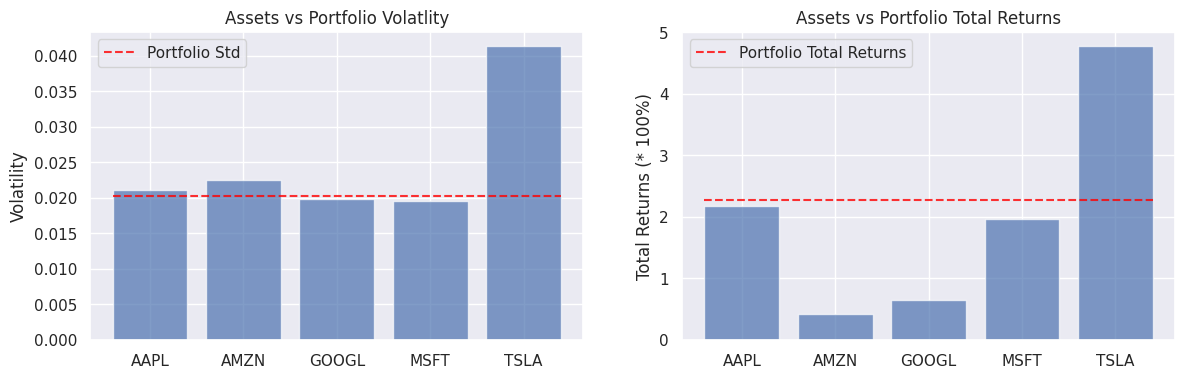
\includegraphics[width=\linewidth,height=0.6\textheight,keepaspectratio]{gfx/m3l1_notes_fig2_assets_vs_portfolio_volatility_returns.png}
\par\smallskip{\small \textbf{Hình 1.2:} Độ lệch chuẩn và tổng lợi suất của từng tài sản so với danh mục đầu tư}
\end{figure}

Trong Hình 1.2, các trọng số chúng ta chọn (ngẫu nhiên) cho ra một danh mục có độ biến động gần với phần lớn các tài sản, nhưng lợi suất lại cao hơn hẳn.

Hãy kiểm tra mối quan hệ giữa phương sai danh mục đầu tư với phương sai của một tài sản ngẫu nhiên, ví dụ MSFT.

\begin{lstlisting}[language=Python,escapeinside={(*@}{@*)}]
# Figure 3
multipliers = np.linspace(0.1,5,100) # (*@Tạo@*) (*@một@*) (*@mảng@*) (*@dùng@*) (*@để@*) (*@nhân@*) (*@với@*) (*@mảng@*) (*@lợi@*) (*@suất@*) MSFT
portfolio_variances = []
msft_variances = []

for multiplier in multipliers:
  temp_returns = r * np.array([1, 1, 1, multiplier, 1]) # (*@Nhân@*) (*@lợi@*) (*@suất@*) MSFT (*@với@*) (*@một@*) (*@con@*) (*@số@*) (*@để@*) (*@thay@*) (*@đổi@*) (*@tuyến@*) (*@tính@*) (*@lợi@*) (*@suất@*), (*@qua@*) (*@đó@*) (*@thay@*) (*@đổi@*) (*@phương@*) (*@sai@*) (*@của@*) MSFT
  temp_port_variance = w.T @ temp_returns.cov() @ w # (*@Tính@*) (*@phương@*) (*@sai@*) (*@danh@*) (*@mục@*) (*@đầu@*) (*@tư@*)
  msft_variances.append((temp_returns['MSFT']).var())
  portfolio_variances.append(temp_port_variance)
  assert np.allclose(r.corr(), temp_returns.corr()) # (*@Với@*) (*@mỗi@*) (*@mảng@*) (*@lợi@*) (*@suất@*) (*@mới@*) (*@mà@*) (*@lợi@*) (*@suất@*) MSFT (*@được@*) (*@nhân@*) (*@với@*) (*@một@*) (*@số@*), (*@các@*) (*@tương@*) (*@quan@*) (*@vẫn@*) (*@giữ@*) (*@nguyên@*)

fig, (ax1, ax2) = plt.subplots(1, 2, figsize = (16,5))

ax1.plot(multipliers, portfolio_variances)
ax1.scatter(1, port_var, color = 'red', label = "Initial Portfolio Variance (non scaled MSFT returns)")
ax1.set_title("Portfolio Variance as MSFT variance is increasing")
ax1.set_xlabel("Multiplier")
ax1.set_ylabel("Variance")
ax1.legend()

ax2.plot(multipliers[10:30], portfolio_variances[10:30])
ax2.scatter(1, port_var, color = 'red', label = "Initial Portfolio Variance (non scaled MSFT returns)")
ax2.plot(multipliers[10:30], msft_variances[10:30], color = 'purple', label = "MSFT Variance (non scaled MSFT returns)")
ax2.set_title("Portfolio Variance vs MSFT variance")
ax2.set_xlabel("Multiplier")
ax2.set_ylabel("Variance")
ax2.legend()

plt.show()
\end{lstlisting}

\begin{figure}[H]
\centering
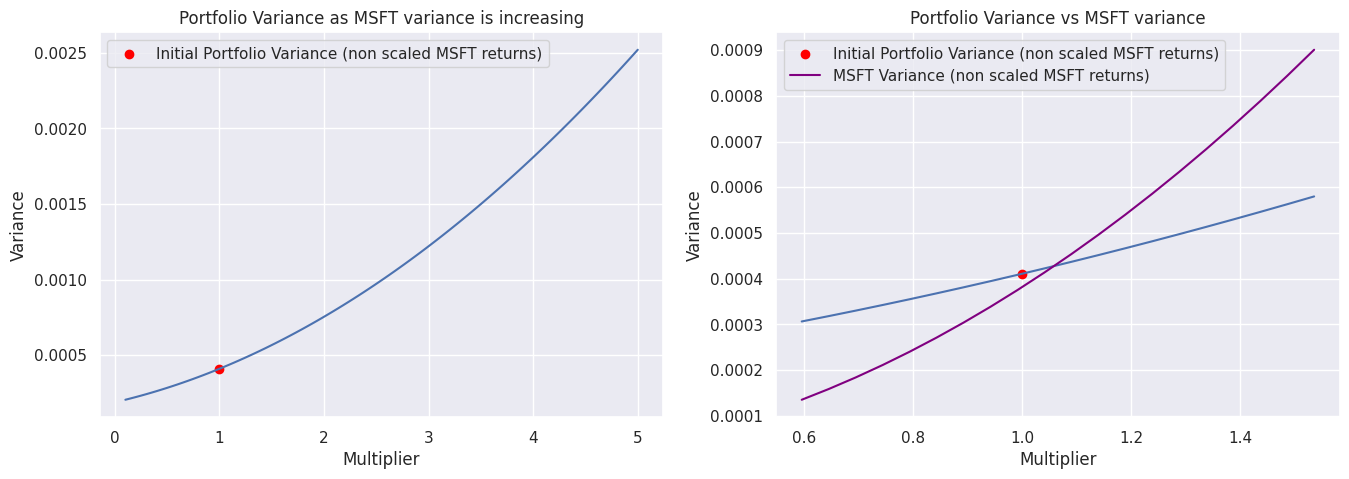
\includegraphics[width=\linewidth,height=0.6\textheight,keepaspectratio]{gfx/m3l1_notes_fig3_portfolio_variance_vs_asset_variance.png}
\par\smallskip{\small \textbf{Hình 1.3:} Phương sai danh mục đầu tư khi phương sai của MSFT tăng dần, so với phương sai của MSFT}
\end{figure}

Hình 1.3 minh họa ảnh hưởng của việc tăng phương sai một tài sản (ở đây là MSFT) lên phương sai danh mục đầu tư. Như dự đoán, mối quan hệ giữa phương sai danh mục đầu tư và phương sai của bất kỳ tài sản nào là bậc hai (đồ thị bên trái). Đồ thị bên phải minh họa sự khác biệt về rủi ro khi nắm giữ một tài sản duy nhất so với nắm giữ cả danh mục đầu tư.

Trong ví dụ tiếp theo, chúng ta giữ nguyên phương sai và trọng số, và xem xét tương quan ảnh hưởng thế nào đến phương sai danh mục đầu tư. Chúng ta giả định $100$ tài sản và xây dựng các ma trận tương quan với tương quan đồng nhất theo từng cặp — nghĩa là mọi cặp tài sản đều có cùng hệ số tương quan. Sự đơn giản hóa này cho phép ta tách biệt ảnh hưởng thuần túy của độ lớn tương quan lên rủi ro danh mục đầu tư. Chúng ta sẽ thử nghiệm $19$ mức tương quan khác nhau, từ $0$ (các tài sản hoàn toàn không tương quan) đến $0.8$ (các tài sản tương quan cao). Lưu ý rằng với $100$ tài sản, các giá trị tương quan nhỏ hơn khoảng $-0.01$ sẽ tạo ra các ma trận tương quan không hợp lệ về mặt toán học (không xác định dương), nên chúng ta tập trung vào phạm vi thực tế từ 0 đến tương quan dương mạnh, đại diện cho các điều kiện thị trường điển hình — từ danh mục đầu tư đa dạng hóa tốt đến các tình huống rủi ro hệ thống cao khi tất cả tài sản có xu hướng di chuyển cùng nhau.

\begin{lstlisting}[language=Python,escapeinside={(*@}{@*)}]
n_assets = 100
w = np.random.dirichlet(np.ones(n_assets), size=1)[0]

degrees_of_freedom = 8
variances = np.random.chisquare(df=degrees_of_freedom, size=n_assets)
variances = variances / np.max(variances) * 0.003
std_devs = np.sqrt(variances)
D = np.diag(std_devs)

# (*@Bắt@*) (*@đầu@*) (*@từ@*) (*@gần@*) (*@bằng@*) (*@0@*) (*@đến@*) (*@tương@*) (*@quan@*) (*@dương@*) (*@cao@*) ((*@phạm@*) (*@vi@*) (*@thực@*) (*@tế@*) (*@của@*) (*@thị@*) (*@trường@*))
correlation_values = np.linspace(0, 0.8, 19)

corr_matrices = []
portfolio_variances = []

for corr in correlation_values:
    # (*@Tạo@*) (*@ma@*) (*@trận@*) (*@tương@*) (*@quan@*) (*@đồng@*) (*@nhất@*)
    R = np.full((n_assets, n_assets), corr)
    np.fill_diagonal(R, 1)

    corr_matrices.append(R)

    # (*@Tính@*) (*@phương@*) (*@sai@*) (*@danh@*) (*@mục@*) (*@đầu@*) (*@tư@*)
    portfolio_variance = w.T @ D @ R @ D @ w
    portfolio_variances.append(portfolio_variance)

# (*@Vẽ@*) (*@biểu@*) (*@đồ@*)
plt.figure(figsize=(10, 5))
plt.plot(correlation_values, portfolio_variances, 'b-o', linewidth=2, markersize=6)
plt.title("Portfolio Variance vs Correlation\n(100 assets, realistic correlation range)")
plt.xlabel("Uniform Pairwise Correlation")
plt.ylabel("Portfolio Variance")
plt.grid(True, alpha=0.3)
plt.xlim(-0.05, 0.85)

plt.show()

print(f"Portfolio variance increases {portfolio_variances[-1]/portfolio_variances[0]:.1f}x as correlation goes from {correlation_values[0]} to {correlation_values[-1]}")
\end{lstlisting}

\begin{lstlisting}[escapeinside={(*@}{@*)}]
Portfolio variance increases 32.7x as correlation goes from 0.0 to 0.8
\end{lstlisting}

\begin{figure}[H]
\centering
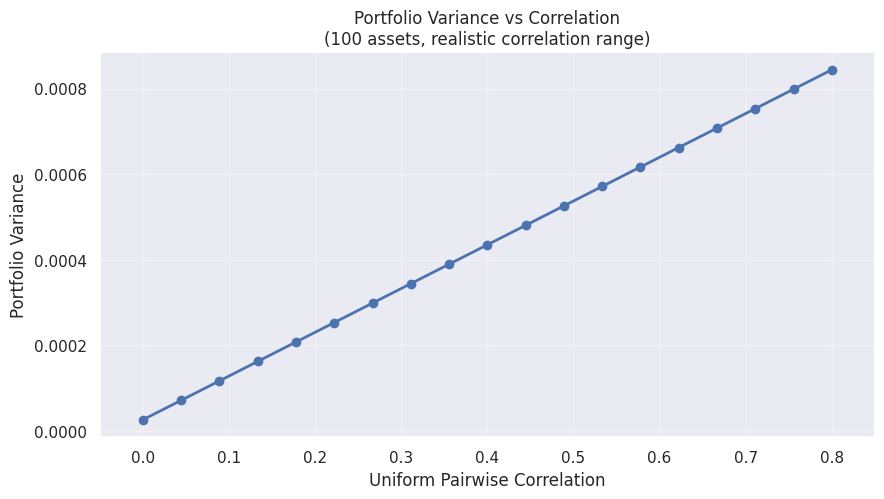
\includegraphics[width=\linewidth,height=0.6\textheight,keepaspectratio]{gfx/m3l1_notes_fig4_portfolio_variance_vs_correlation.png}
\par\smallskip{\small \textbf{Hình 1.4:} Phương sai danh mục đầu tư theo tương quan (100 tài sản, phạm vi tương quan thực tế)}
\end{figure}

Những học viên chưa có nền tảng tài chính có thể không ngờ tới kết quả này. Ngay cả khi phương sai từng tài sản và trọng số không đổi, sự thay đổi trong tương quan vẫn ảnh hưởng mạnh mẽ đến phương sai danh mục đầu tư. Cụ thể trong ví dụ này, phương sai danh mục đầu tư thấp nhất khi tương quan bằng 0 (các tài sản không tương quan), và tăng tuyến tính khi tương quan trở nên dương hơn. Với tương quan $0.8$, phương sai danh mục đầu tư cao gấp khoảng $36$ lần so với khi tương quan bằng 0. Điều này minh họa nguyên lý nền tảng của đa dạng hóa: kết hợp các tài sản không tương quan giúp giảm rủi ro hiệu quả hơn nhiều so với kết hợp các tài sản tương tự, có tương quan cao. Mối quan hệ tuyến tính quan sát được (với tương quan đồng nhất) sẽ trở nên phức tạp hơn khi cấu trúc tương quan thực tế hơn, nhưng thông điệp cốt lõi vẫn đúng — khi các tài sản tương quan cao hơn, lợi ích đa dạng hóa giảm dần và rủi ro danh mục tăng lên. Điều này giải thích tại sao các cuộc khủng hoảng thị trường lại nguy hiểm đối với các danh mục đầu tư đa dạng hóa: trong giai đoạn căng thẳng, tương quan có xu hướng tăng vọt lên gần $1$, khiến các danh mục tưởng chừng đa dạng hóa tốt lại hành xử gần như một tài sản đơn lẻ.

\textbf{Bài tập 10:}

Chọn $n \geq 2$ cổ phiếu/trái phiếu và xây dựng một danh mục đầu tư (chọn trọng số phù hợp) sử dụng dữ liệu lịch sử sao cho phương sai danh mục bằng $0$ (hoặc thực sự gần $0$ để được coi là $0$) và lợi suất dương (khác xa $0$). Trình bày phát hiện của bạn trên diễn đàn. Nếu bạn không tìm được, hãy trình bày lý do vì sao không tìm được.

\section{Trọng số Danh mục Đầu tư}

Giả sử ta có thể xây dựng một danh mục đầu tư gồm cổ phiếu, trái phiếu và tiền điện tử. Một nhà đầu tư có thể chọn nắm giữ nhiều trái phiếu trong khi người khác chọn chủ yếu cổ phiếu và người thứ ba lại yêu thích tiền điện tử. Sự lựa chọn này liên quan đến hồ sơ rủi ro của nhà đầu tư; nói cách khác, việc chọn trọng số sẽ đáp ứng nhu cầu về lợi suất cụ thể với một mức chấp nhận rủi ro (phương sai) nhất định.

Từ góc nhìn này, việc chọn trọng số là một vấn đề mang tính chủ quan, và trên thực tế, các nhà đầu tư hành xử rất khác nhau (Elton et al.). Một trong những cách tốt nhất để khám phá điều này là xây dựng đồ thị Đường biên Hiệu quả (Efficient Frontier).

\begin{lstlisting}[language=Python,escapeinside={(*@}{@*)}]
from scipy.optimize import minimize

weights = np.random.dirichlet(np.ones(5)*0.7, size = 20000) # (*@Tạo@*) 20000 (*@bộ@*) (*@trọng@*) (*@số@*) (*@sử@*) (*@dụng@*) (*@phân@*) (*@phối@*) dirichlet

assert np.isclose(np.sum(weights, axis = 1), 1).all() # (*@Kiểm@*) (*@tra@*) (*@mỗi@*) (*@bộ@*) (*@trọng@*) (*@số@*) (*@có@*) (*@tổng@*) (*@bằng@*) 1

eff_front_dict = {}
cov_matrix_ret = r.cov() * 252
expected_returns = r.mean() * 252

# (*@Điền@*) (*@vào@*) eff_front_dict
for w in weights:
  port_ret = expected_returns @ w.T # (*@Lợi@*) (*@suất@*) (*@kỳ@*) (*@vọng@*) (*@chuẩn@*) (*@hóa@*) theo (*@năm@*)
  port_std = np.sqrt(w.T @ cov_matrix_ret @ w)
  eff_front_dict[str(list(w))] = [port_ret, port_std]

eff_frontier_dataframe = pd.DataFrame(eff_front_dict, index = ['Returns', 'Standard Deviation']).T # (*@Lưu@*) (*@mọi@*) (*@thứ@*) (*@vào@*) (*@một@*) dataframe

def get_portfolio_stats(weights, expected_returns, cov_matrix):
    port_ret = expected_returns @ weights
    port_std = np.sqrt(weights.T @ cov_matrix @ weights)
    return port_ret, port_std

def negative_sharpe_ratio(weights, expected_returns, cov_matrix, risk_free_rate=0.02):
    port_ret, port_std = get_portfolio_stats(weights, expected_returns, cov_matrix)
    sharpe_ratio = (port_ret - risk_free_rate) / port_std
    return -sharpe_ratio

def minimum_variance(weights, expected_returns, cov_matrix):
    return get_portfolio_stats(weights, expected_returns, cov_matrix)[1]

def efficient_frontier_point(expected_returns, cov_matrix, target_return):
    n_assets = len(expected_returns)
    args = (expected_returns, cov_matrix)
    constraints = (
        {'type': 'eq', 'fun': lambda w: np.sum(w) - 1},
        {'type': 'eq', 'fun': lambda w: get_portfolio_stats(w, expected_returns, cov_matrix)[0] - target_return}
    )
    bounds = tuple((0, 1) for _ in range(n_assets))

    result = minimize(
        minimum_variance,
        x0=np.ones(n_assets) / n_assets,
        args=args,
        method='SLSQP',
        bounds=bounds,
        constraints=constraints
    )

    return result.x

def get_efficient_frontier(expected_returns, cov_matrix, n_points=100):
    # (*@Tìm@*) (*@danh@*) (*@mục@*) (*@phương@*) (*@sai@*) (*@nhỏ@*) (*@nhất@*)
    n_assets = len(expected_returns)
    args = (expected_returns, cov_matrix)
    constraints = ({'type': 'eq', 'fun': lambda w: np.sum(w) - 1})
    bounds = tuple((0, 1) for _ in range(n_assets))

    min_var_result = minimize(
        minimum_variance,
        x0=np.ones(n_assets) / n_assets,
        args=args,
        method='SLSQP',
        bounds=bounds,
        constraints=constraints
    )
    min_ret, min_std = get_portfolio_stats(min_var_result.x, expected_returns, cov_matrix)

    # (*@Tìm@*) (*@danh@*) (*@mục@*) (*@lợi@*) (*@suất@*) (*@lớn@*) (*@nhất@*)
    max_ret_idx = np.argmax(expected_returns)
    max_ret = expected_returns[max_ret_idx]

    # (*@Tạo@*) (*@các@*) (*@điểm@*) (*@trên@*) (*@đường@*) (*@biên@*) (*@hiệu@*) (*@quả@*)
    target_returns = np.linspace(min_ret, max_ret, n_points)
    efficient_portfolios = []

    for target_return in target_returns:
        weights = efficient_frontier_point(expected_returns, cov_matrix, target_return)
        ret, std = get_portfolio_stats(weights, expected_returns, cov_matrix)
        efficient_portfolios.append([std, ret])

    return np.array(efficient_portfolios)

# (*@Tính@*) (*@các@*) (*@điểm@*) (*@của@*) (*@đường@*) (*@biên@*) (*@hiệu@*) (*@quả@*)
efficient_points = get_efficient_frontier(expected_returns, cov_matrix_ret)

# (*@Vẽ@*) (*@biểu@*) (*@đồ@*)
plt.figure(figsize=(10,6))
plt.scatter(x=eff_frontier_dataframe['Standard Deviation'],
           y=eff_frontier_dataframe['Returns'],
           alpha=0.4)
plt.scatter(x=r.std() * np.sqrt(252),
           y=expected_returns,
           color='red',
           label="Individual Assets",
           alpha=0.7)
plt.plot(efficient_points[:,0],
         efficient_points[:,1],
         'orange',
         linewidth=3,
         label='Efficient Frontier',
         alpha=0.6)
plt.title("Efficient Frontier")
plt.xlabel("Annual Portfolio Standard Deviation")
plt.ylabel("Annual Portfolio Returns")
plt.legend()
plt.grid(True)
plt.show()
\end{lstlisting}

\begin{figure}[H]
\centering
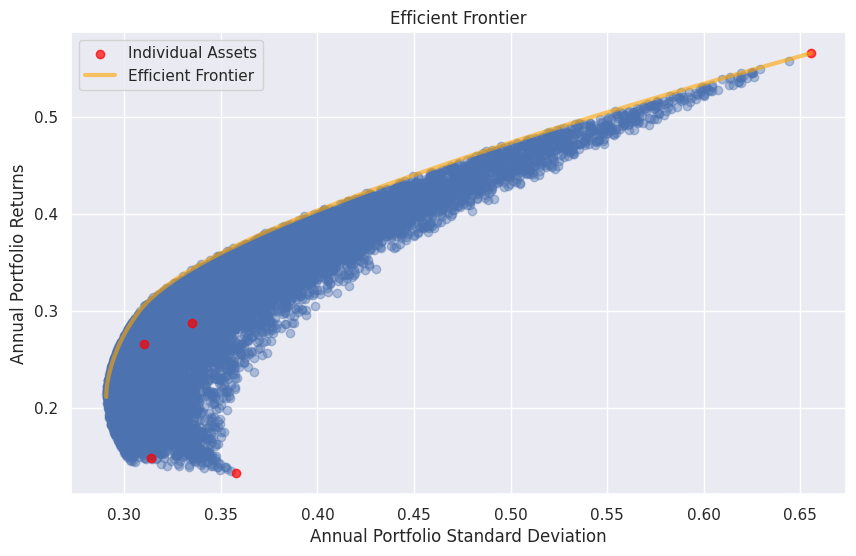
\includegraphics[width=\linewidth,height=0.6\textheight,keepaspectratio]{gfx/m3l1_notes_fig5_returns_vs_risk_portfolios.png}
\par\smallskip{\small \textbf{Hình 1.5:} Đường biên Hiệu quả (Efficient Frontier) của danh mục đầu tư gồm 5 tài sản}
\end{figure}

Hãy đọc hiểu minh họa trên, được thừa nhận là một trong những đồ thị quan trọng nhất trong quản lý danh mục đầu tư.

Trước hết, ta cần quan sát hình dạng của đường biên: đường cong trải dài ở phần trên bên trái của biểu đồ phân tán đại diện cho tất cả các danh mục đầu tư tối ưu khả dĩ, mang lại lợi suất kỳ vọng cao nhất cho một mức rủi ro cho trước (hoặc rủi ro thấp nhất cho một mức lợi suất kỳ vọng cho trước). Đường cong này được gọi là \textbf{đường biên hiệu quả} (efficient frontier).

Thứ hai, nếu vẽ các đường thẳng đứng trên đồ thị này, mỗi đường sẽ cắt đường biên tại một điểm đại diện cho danh mục có lợi suất cao nhất ứng với mức rủi ro cụ thể đó. Đồng thời, có rất nhiều bộ trọng số khiến danh mục chịu cùng mức rủi ro nhưng lợi suất thấp hơn. Điều đó nên khiến ta chú ý rằng mặc dù trọng số mang tính chủ quan, nếu danh mục mà nhà đầu tư chọn không nằm trên đường biên hiệu quả, thì nhà đầu tư có thể đạt lợi suất tốt hơn bằng cách đi theo đường thẳng đứng lên trên cho đến khi chạm đường biên hiệu quả. Nói ngắn gọn, với bất kỳ mức rủi ro (phương sai) nào, luôn tồn tại một cấu trúc danh mục tối ưu tối đa hóa lợi suất.

Điều tương tự cũng đúng nếu ta vẽ các đường ngang. Trong trường hợp này, ta có thể khẳng định rằng với bất kỳ mức lợi suất nào, ta có thể tối thiểu hóa rủi ro bằng cách đi theo đường ngang sang trái cho đến khi cắt đường biên hiệu quả.

Khi di chuyển lên trên và sang phải dọc theo đường biên, ta thấy lợi suất tiềm năng cao hơn nhưng cũng rủi ro cao hơn. Điều này minh họa nguyên lý nền tảng rằng để đạt lợi suất cao hơn, nhìn chung ta phải chấp nhận rủi ro cao hơn. Hình dạng lõm của đường biên minh họa lợi ích của đa dạng hóa. Các danh mục nằm trên đường biên thường được đa dạng hóa tốt, mang lại hồ sơ rủi ro-lợi suất tốt hơn so với từng tài sản riêng lẻ.

\textbf{Bài tập 11:}

Xây dựng danh mục đầu tư của riêng bạn, theo sở thích của bạn: chọn một hoặc nhiều cổ phiếu, ETF, trái phiếu và tiền điện tử. Cố gắng bao gồm các tài sản không tương quan nhiều với phần còn lại của danh mục (nếu có thể) và cũng bao gồm một số tài sản có độ biến động rất cao (altcoin vốn hóa lớn hoặc mới phát hành). Sử dụng mã đã cung cấp ở trên để xây dựng đường biên hiệu quả. Dán đồ thị lên diễn đàn cùng với một đoạn văn \textbf{ngắn} liệt kê các tài sản đã chọn.

\textbf{Bài tập 12 (Tùy chọn):}

Trong đoạn đầu tiên của notebook này, chúng ta đã đề cập rằng với $n$ vector $r_{i}$, khi không có đa cộng tuyến, ta có $\text{dim}(\text{span}(r_{i})) = n$. Ngược lại, số chiều của $\text{span}$ sẽ thấp hơn $n$. Đây là một kết quả đã biết trong đại số tuyến tính. Hãy dùng giáo trình đại số tuyến tính yêu thích của bạn để ôn lại khái niệm đa cộng tuyến, sau đó lập luận vì sao một nhà đầu tư vẫn giữ một tài sản trong danh mục khi tài sản đó có thể được viết dưới dạng tổ hợp tuyến tính hoàn hảo của các tài sản còn lại trong danh mục. Nhà đầu tư có nên loại bỏ tài sản đó không? Đóng góp của nó vào việc giảm phương sai danh mục hoặc tăng lợi suất là gì? Nó có mang lại sự linh hoạt trong quản lý danh mục hay không?

\textbf{Bài tập 13:}

Xuyên suốt bài học này, học viên đã được giới thiệu cách sử dụng đúng trung bình số học và trung bình hình học. Trong mục \emph{2.4 Chuẩn hóa Lợi suất theo Năm}, chúng ta đã giải thích cách chuẩn hóa lợi suất phần trăm và lợi suất log theo năm nếu cần hiệu ứng lãi kép. Tuy nhiên, khi xây dựng đường biên hiệu quả, ta đã làm như sau: \texttt{expected\_returns = r.mean() * 252}. Tại sao? Trong câu trả lời của bạn, hãy xem xét bối cảnh tối ưu hóa danh mục đầu tư và liệu ta đang tập trung mô hình hóa lợi suất kỳ vọng cho mục đích thống kê hay tính mức tăng trưởng lịch sử thực tế của một khoản đầu tư do lãi kép. Thảo luận về hệ quả của việc sử dụng trung bình số học trong ngữ cảnh này.

\section{Kết luận}

Trong bài học này, chúng ta đã học rằng lợi suất logarit có tính cộng dồn và hữu ích cho phân tích dài hạn, trong khi lợi suất phần trăm trực quan hơn cho đánh giá hiệu suất ngắn hạn. Chúng ta cũng đã tìm hiểu cách chuẩn hóa lợi suất theo năm, cho phép so sánh công bằng giữa các khoản đầu tư có khung thời gian khác nhau.
Bài học nhấn mạnh tầm quan trọng của việc hiểu phương sai danh mục đầu tư và các thành phần của nó. Chúng ta đã thấy phương sai từng tài sản, trọng số và tương quan đều đóng vai trò quan trọng trong việc xác định rủi ro tổng thể của danh mục. Khái niệm đường biên hiệu quả minh họa sự đánh đổi giữa rủi ro và lợi suất, làm nổi bật lợi ích của đa dạng hóa.

Thông qua các ví dụ và bài tập thực hành bằng Python, chúng ta đã có kinh nghiệm thực tế trong việc tính toán và diễn giải các chỉ số này. Kiến thức này tạo nền tảng thiết yếu cho các chủ đề nâng cao hơn trong quản lý danh mục đầu tư và phân tích tài chính.

\textbf{Tài liệu tham khảo}

\begin{itemize}
  \item Elton, Edwin J., et al. \emph{Modern Portfolio Theory and Investment Analysis}. John Wiley \& Sons, 2009.
  \item Ruppert, David, and David S. Matteson. \emph{Statistics and Data Analysis for Financial Engineering}. 2nd ed., Springer, 2011.
\end{itemize}
